%!TEX root = ../report.tex

%
% Introduction
%

\section{Introduction}
\label{sec:introduction}

% General description of the problem and its context, current 
% solutions, and road map of the project.
% 2 - 3 pages
% TODO: Mobile proximity based apps (Special kind of context aware), Explain context-aware, Examples
% Technologies to know if the user is nearby some POI
% Development of proximity-based apps
% Smart spaces
% TODO: What are native and web mobile apps
% TODO: What makes more sense to proximity-based apps
% (Native vs Web)
% This paper is about...
% Present next sections

% Problem
The use of context-aware mobile applications (apps)
has been increasing.
These apps use context, acquired
from one or more sensors and other user's data, 
such as the calendar. For instance, it is possible to
build an app that puts the phone in silent mode if the
user is in a meeting. Proximity-based apps are
context-aware apps that allow the user to interact
with the app if he is nearby some point of interest (POI).
Table \ref{tab:app_comparison} shows some statistics
about the most popular apps in Google Play Store,
including examples of proximity-based apps,
such as Foursquare\footnote{https://foursquare.com},
Skout\footnote{http://www.skout.com/} and
Tinder\footnote{http://www.gotinder.com/}

\begin{table}[h]
\centering
\begin{tabular}{|c|r|r|}
\hline
\textbf{App} & \multicolumn{1}{c|}{\textbf{Nr of Downloads}} & \multicolumn{1}{c|}{\textbf{User Rating (0 to 5)}} \\ \hline
Facebook & 1-\num{5e9} & 4.0 \\ \hline
Twitter & 1-\num{5e8} & 4.1 \\ \hline
Instagram & 1-\num{5e8} & 4.5 \\ \hline
Foursquare & 1-\num{5e7} & 4.1 \\ \hline
Skout & 1-\num{5e7} & 4.1 \\ \hline
Tinder & 1-\num{5e7} & 4.1 \\ \hline
\end{tabular}
\caption{Some statistics about most used apps including some
proximity-based ones in Google Play Store. 
Source: App Annie (http://www.appannie.com/) 
in 2, December, 2014}
\label{tab:app_comparison}
\end{table}

Facebook is the app with the
greatest number of downloads.
It has, at least, \num{1e9}. Twitter and Instagram
have, at least, \num{1e8} downloads.
One of the 
proximity-based apps has, at least, \num{1e7} downloads.
Which means, one of
the proximity-based apps represents
1/100 of Facebook's downloads and 1/10 of Twitter's
and Instagram's downloads. In terms of rating, all apps
have similar values

% Possible solutions
To know if the user is nearby some point of interest,
we need to know the user's location. We can use 
the Global Positioning System 
(GPS)\cite{masumoto1993global} to
get this information. Most apps use this technology 
because most smartphones have a GPS receiver. 
%Show some statistics about smartphones with GPS
Unfortunately, GPS cannot be used indoors because 
the signal can
be very weak inside a building. To make proximity-based
apps work properly indoors, we need to use other 
technologies.

%-----------------------------
% BLE
%-----------------------------
\subsection{BLE}
\label{sub:bluetooth_low_energy}
Bluetooth is a wireless, short-range, communication technology.
Bluetooth Low Energy (BLE)\footnote{http://www.bluetooth.com/Pages/Bluetooth-Smart.aspx} 
is an improvement of classic Bluetooth since it consumes 
very low power, allowing it to be used by smaller devices.
And that is the main reason for this technology to start to 
be used for proximity-based mobile apps,

BLE Beacons are devices, that use BLE, to broadcast a 
Universally Unique Identifier (UUID). 
These devices use the 
iBeacon\footnote{http://developer.apple.com/ibeacon/} 
protocol, which was created
by Apple\texttrademark. In this protocol the beacons
advertise the following sets of bytes:
\begin{description}
  \item[UUID] has 16 bytes and it is used to differentiate a 
  large group of related beacons
  \item[Major] has 2 bytes and it is used to distinguish a smaller 
  subset of beacons within the larger group
  \item[Minor] has 2 bytes and it is used to distinguish individual
  beacons within the smaller subset
\end{description}
A smartphone that
has BLE can get this signal with the mentioned bytes.
But, only smartphones
with Bluetooth, at least, version 4, have BLE.

For instance, a store owner wants to advertise a promotion
to potential customers that are nearby his store. To 
achieve this goal, the store owner would need to put
a beacon inside his store and his customers would need an
app that would get the beacon's signal and show a 
notification in the customers' smartphones,
as shown in figure \ref{fig:store_example}.
\begin{figure}[!ht]
  \centering
    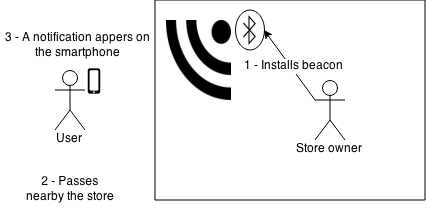
\includegraphics[width=0.9\textwidth]{img/store_example}
    \caption{Interaction between the user's smartphone
    and a beacon inside a store}
    \label{fig:store_example}
\end{figure}

To develop apps that use beacons, the 
BLE API can be used, provided by the 
mobile platform or simply by the Software
Development Kit (SDK) from the 
beacons vendor. The example of the store owner is a
simple one. The app just gets the signal and shows a 
notification. However, if the store owner has more than
one store and wants to show a different promotion depending
on each store, the app would need to do more than just get
the beacon's signal. After getting the signal, the app
would get the promotion data for that beacon, from a 
backend. The developer of this app, would need to
write the code that gets the beacon's signal and also
the code that will get the information from the backend.

Another example could be an app for a museum. The owner
of a museum wants to show information regarding the
exhibition, in the 
visitors' smartphones, about the pieces that are in a given
room. He would need one beacon for each piece and an app
that would get the beacon's signal and use a
backend to get the right information about a given piece.
The museum needs to advertise, to its visitors, that such
an app exists and also, tell them to download the app
before they enter the museum. For both scenarios the developers will have to write similar code to get
the beacon's signal and get data from a backend.

%-----------------------------
% Smart Places
%-----------------------------
\subsection{Smart Places}
\label{sub:smart_places}
Before going further, we will introduce the concept of
Smart Place, which is a place that can, somehow,
interact with users nearby and then allows 
users to interact 
with it.
In this context, a Smart Place have beacons and the users
have apps, installed in their smartphones, 
that can interact
with them and show relevant information to the user.
With this definition, we can say, for instance
that the owner of the store, wants to
turn his store into a Smart Place.
The same applies to the museum owner.
The user would need to install two apps, one for the
store and another one for the museum.
If there is another Smart Place, the user would need to
install another app.

Any mobile app can be a native or a web app. Native apps
are apps that we have to install and that can access
device's features, such as BLE. Web apps are web
applications, designed for mobile devices, that run
on the device's browser. Table \ref{tab:native_vs_web}
compares some characteristics of both kinds of apps.
% Table Native vs web
\begin{table}[h]
\centering
\begin{tabular}{|c|c|c|l}
\cline{1-3}
 & Native & Web &  \\ \cline{1-3}
\begin{tabular}[c]{@{}c@{}}Access to device's features \\ (Camera, accelerometer,etc)\end{tabular} & All & Limited &  \\ \cline{1-3}
Installation needs & \begin{tabular}[c]{@{}c@{}}Need to install\\ the app\end{tabular} & \begin{tabular}[c]{@{}c@{}}Only a web browser\\ is needed\end{tabular} &  \\ \cline{1-3}
\begin{tabular}[c]{@{}c@{}}Method for finding\\ the app\end{tabular} & App stores & \begin{tabular}[c]{@{}c@{}}Users have to find\\ it somewhere\end{tabular} &  \\ \hline
Updates & \begin{tabular}[c]{@{}c@{}}Users can choose\\ to not update the\\ app\end{tabular} & \begin{tabular}[c]{@{}c@{}}All users have\\ access to the same\\ version\end{tabular} &  \\ \cline{1-3}
Where it can run & \begin{tabular}[c]{@{}c@{}}Only on the platform\\ for which it was\\ developed for\end{tabular} & On any platform &  \\ \cline{1-3}
\end{tabular}
\caption{A comparison of some characteristics of Native and Web mobile apps}
\label{tab:native_vs_web}
\end{table}

Mobile web apps do not need to be
installed but they do not have access
to same device's features that native apps have.
Mobile apps for Smart Places, according to our definition,
need to be native, because we need to get signals from
nearby beacons. For that, we need to use bluetooth, which is
not available in web apps, since they run in the browser.
A solution to allow developers to get the best of both sides
is proposed here: On one side,
native apps can detect nearby beacons. On the other side,
web apps do not need to be installed.

%-----------------------------
% Framework
%-----------------------------
\subsection{Framework}
\label{sub:framework}
% Solution being proposed here aims to
% Users: Interact with any Smart Place
% withou downloading one app for each one
% Developers: Develop apps based on POIs
% using web technologies
% Android app for users, owners
% Backend for...
% Alternative to QR Code without need of scanning
The solution being proposed here aims to allow
users to interact with any Smart Place without
the need of download and install one native
app, in their mobile devices, for each Smart
Place.
Developers will be able to develop their
applications, that are based on POIs, using
web technologies, such as HTML, CSS and Javascript
and they will not need to write code related with
the BLE beacons neither the backend where the data,
for each POI, is stored.
To achieve this goal, an Android app will be part
of the solution. This mobile app will be developed
to be used by users and by people who own a space
and want to install beacons in their spaces to
offer some kind of interaction.

QR Codes already provide a similar solution to
deliver content to mobile devices.
However, the user needs to see the code printed
somewhere and scan it using an app to read
this kind of codes.
Also, they only allow the user to receive content,
such as, a web page or a link to a video.
This project can be considered as an alternative
to QR Codes but without requiring the user
to scan any code. The only requirement is that
the user needs to turn on the Bluetooth receiver
of his mobile device.

In next section, we describe the main
objectives of the project being proposed.
Section \ref{sec:related_work} describes related
work about some examples of apps that use BLE Beacons
and the development and deployment of
context-aware mobile apps.
In section \ref{sec:architecture} the architecture of our
solution is explained, 
its main components and the role of
each one.
Section \ref{sec:evaluation} is about how the solution
will be evaluated.
Finally, section \ref{sec:conclusions} has a summary of
the main ideas of the entire document.
